
% 
% Annual Cognitive Science Conference
% Sample LaTeX Paper -- Proceedings Format
% 

% Original : Ashwin Ram (ashwin@cc.gatech.edu)       04/01/1994
% Modified : Johanna Moore (jmoore@cs.pitt.edu)      03/17/1995
% Modified : David Noelle (noelle@ucsd.edu)          03/15/1996
% Modified : Pat Langley (langley@cs.stanford.edu)   01/26/1997
% Latex2e corrections by Ramin Charles Nakisa        01/28/1997 
% Modified : Tina Eliassi-Rad (eliassi@cs.wisc.edu)  01/31/1998
% Modified : Trisha Yannuzzi (trisha@ircs.upenn.edu) 12/28/1999 (in process)
% Modified : Mary Ellen Foster (M.E.Foster@ed.ac.uk) 12/11/2000
% Modified : Ken Forbus                              01/23/2004
% Modified : Eli M. Silk (esilk@pitt.edu)            05/24/2005
% Modified : Niels Taatgen (taatgen@cmu.edu)         10/24/2006
% Modified : David Noelle (dnoelle@ucmerced.edu)     11/19/2014
% Modified : Elisa Kreiss (ekreiss@uos.de)    10/10/2016

%% Change ''letterpaper'' in the following line to ''a4paper'' if you must.

\documentclass[10pt,letterpaper]{article}

\usepackage{cogsci}
\usepackage{pslatex}
\usepackage{apacite}
\usepackage{amsmath,amssymb}
\usepackage{graphicx}
\usepackage{color}
\usepackage{url}
\usepackage{todonotes}
\usepackage{mathtools}
\usepackage{stmaryrd}
\usepackage{booktabs}
\usepackage{array}

\newcommand{\den}[2][]{
\(
\left\llbracket\;\text{#2}\;\right\rrbracket^{#1}
\)
}

%\newcommand{\url}[1]{$#1$}


\definecolor{Blue}{RGB}{0,0,255}
\definecolor{Green}{RGB}{10,200,100}
\definecolor{Red}{RGB}{255,0,0}
\newcommand{\jd}[1]{\textcolor{Blue}{[jd: #1]}}  
\newcommand{\rdh}[1]{\textcolor{Red}{[rdh: #1]}}  
\newcommand{\red}[1]{\textcolor{Red}{#1}}
\newcommand{\ndg}[1]{\textcolor{Green}{[ndg: #1]}}

 \newcommand{\denote}[1]{\mbox{ $[\![ #1 ]\!]$}}


\newcommand{\subsubsubsection}[1]{{\em #1}}
\newcommand{\eref}[1]{(\ref{#1})}
\newcommand{\tableref}[1]{Table \ref{#1}}
\newcommand{\figref}[1]{Fig.~\ref{#1}}
\newcommand{\appref}[1]{Appendix \ref{#1}}
\newcommand{\sectionref}[1]{Section \ref{#1}}

\title{Mentioning atypical properties of objects is communicatively efficient}

 
\author{{\large \bf Elisa Kreiss, Judith Degen, Robert X.D. Hawkins, Noah D.~Goodman} \\
  ekreiss@uos.de, \{jdegen,rxdh,ngoodman\}@stanford.edu\\
  Department of Psychology, 450 Serra Mall \\
  Stanford, CA 94305 USA}



\begin{document}

\maketitle


\begin{abstract}

\jd{write once modeling results clear}

\textbf{Keywords:} 
keywords
\end{abstract}

%\section{\bf Introduction}

Reference to objects is one of the most basic functions of language. How do speakers decide which of an object's properties to include in a referring expression? This problem of content selection (\jd{cite the dutch}) has plagued cognitive science for decades. For example, in Fig.~1c, the utterances `blue banana', `banana', `blue fruit', etc.~all uniquely establish reference to the same target: the blue banana. How do speakers decide between these? One factor that has been identified as affecting speakers' choice of referring expression is the expression's \emph{contextual informativeness}. Assuming that properties either do or do not apply to objects, `banana' would be the appropriate choice in Fig.~1c (where no other banana competes with the target banana), but `blue banana' when there is also a competing brown banana (as in Fig.~1b). However, previous research has established that this is not the case: speakers generally prefer to mention properties of objects to the extent that they are atypical, even when doing so is unnecessary for uniquely establishing reference \cite{sedivy2003a, Mitchell2013, westerbeek2015, rubiofernandez2016}. That is, speakers are more likely to redundantly call a blue banana `blue banana' but a yellow banana simply `banana'. Why is this so?

%The banana itself is a color-diagnostic object (Tanaka and Presnell, 1999), meaning different colors can have differently strong associations with, or be differently symptomatic of the object. A banana is normally associated with being yellow, a bit less with being brown, and not at all with being blue. When rating the association between the object and its color, we talk about \textit{typicality}. For a cup, all colors have approximately the same typicality, and it is therefore a non-color-diagnostic object.\\

%Various studies (Westerbeek, Mitchell, …) have shown that the color of a color-diagnostic object governs the chosen referring expression significantly. Westerbeek (cite) looked at contexts in which the referred-to object can unambiguously be distinguished from the other objects by only mentioning the type. Additionally, there has always been one object present that had the same color as the target (similar to Fig.~1d). Therefore, only considering unambiguous reference expressions, the use of color terms in any way would be “overinformative”, i.e., a true but unnecessarily added information. Westerbeek (cite) found that the lower the typicality for a color given the referred-to object is, the more likely one is to mention the color overinformatively.\\

%Looking at the example from the beginning again, Westerbeek's result would suggest that people would also tend to say 'blue banana'  in Fig.~1c to refer to the target object even if 'banana' would already be a sufficient way to do so.\\

An account of why more typical properties are less likely to be mentioned is still lacking. Some (\jd{cite}) have proposed that it is due to a speaker-internal pressure to mention salient properties; others (\jd{cite}) have proposed that speakers mention properties to facilitate the listener'��s visual search. Here, we ask the computational-level question: when should a rational speaker with the goal of correctly communicating the intended referent be expected to mention an object's color?

Following the bulk of the previous literature, we assume that a speaker's choice of referring expression is governed by multiple factors, including the expression's contextual informativeness and its cost. Following  \citeA{GrafEtAl2016,DegenEtAl-inprep} \jd{who else?}, we model speaker behavior formally within the Rational Speech Act (RSA) framework \cite{frank2012, GoodmanFrank2016}. However, we show that with a deterministic semantics for nouns and color adjectives, RSA cannot capture typicality effects in language. Therefore, also following \citeA{GrafEtAl2016,DegenEtAl-inprep}, we allow the semantics of expressions to assume a continuous value. That is, we allow `banana'-hood or `blue'-ness to apply to a given object to some degree rather than deterministically. This change directly affects expressions' contextual informativeness, resulting in precisely the expected typicality effects, as we demonstrate below.

In order to quantitatively evaluate the model, we collected freely produced referring expressions to objects in a web-based two-player reference game experiment (see \figref{fig:mturk}). We presented participants with color-diagnostic objects that varied in how typical their colors were. Objects were presented in different contexts to vary the contextual informativeness of mentioning color (see \figref{fig:contexts}). 

%One of the two players was given the role of the listener, the other one the role of the speaker. They could communicate freely with each other through a chat box which ensured natural language data. In each context, both saw the same objects but only the speaker had the special marking of the referent which he had to communicate to the listener. The listener then had to deduce the correct target from the speaker’s utterance and mark it by clicking on the object. 
%The context were manipulated by a differing typicality for the target object, and by distractor variation (either sharing the target's type, color or none of those). This way we could evaluate the effect of typicality and different kinds of contexts on referring expressions.

We expected to replicate color typicality effects on referring expressions in at least those contexts where color use would be `overinformative' (Fig.~1c) and 1d)), i.e., not strictly necessary for uniquely establishing reference. We also included control contexts in which mentioning color was informative (Fig.~1a) and 1b)). In these conditions, it is necessary to mention an object's color to unambiguously establish reference. Thus, we can test for typicality effects even in situations where mentioning color is seemingly necessary.

\begin{figure}
	\centering
	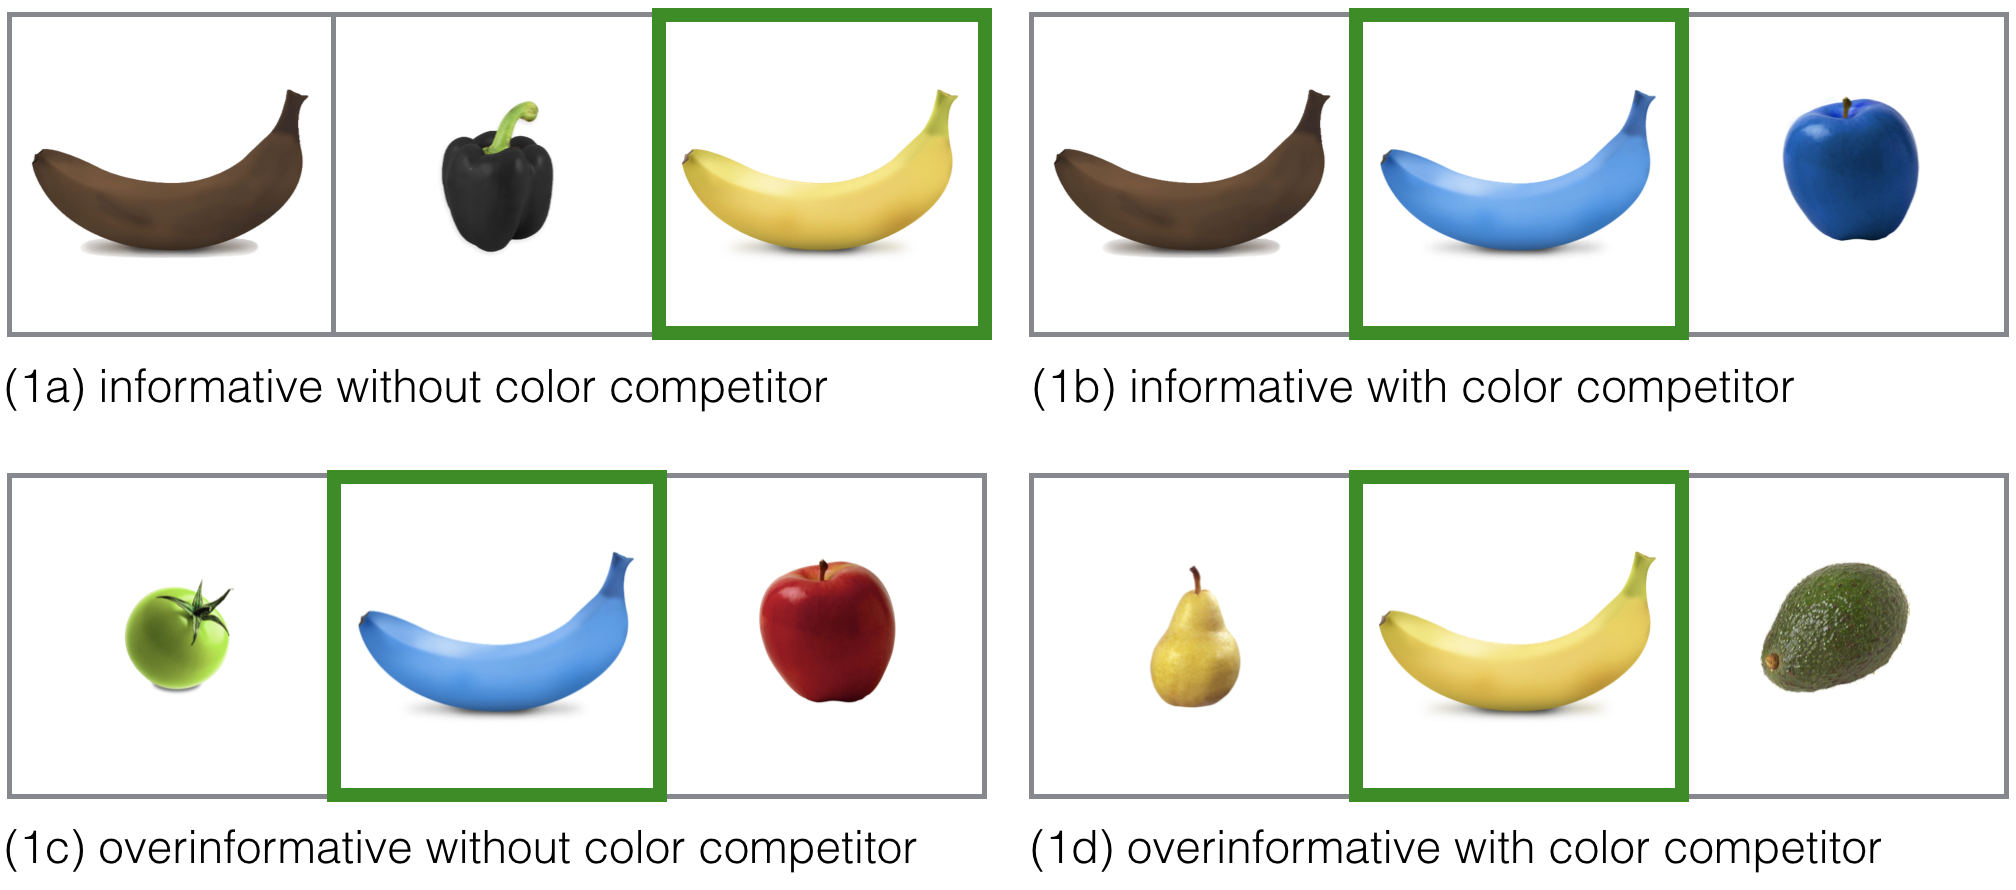
\includegraphics[width=.5\textwidth]{graphs/context_overview}
	\caption{The four context conditions, exemplified by the \textit{banana} domain. The target is outlined in green; the color and type of the distractors differ with each condition (see text). \jd{elisa: please make this figure with exactly the same labels as in  results Figure 4 (informative, informative-cc, etc, and explain in figure caption -- in making labels shorter, also make them more legible or we'll be rejected outright for illegible figures.}
	}
	\label{fig:contexts}
\end{figure}

We begin by reporting the production experiment, including norming studies we conducted to empirically elicit typicality values for all utterance-object pairs. We then report a comparison of different RSA models with graded semantics against a deterministic semantics baseline. Model comparison makes use of the empirically elicited typicality values to derive behavioral predictions, which we compare against the data obtained in the reported production experiment.

%In this paper, we also describe how this effect can be modeled by using the Rational-Speech-Acts (RSA) framework (Frank \& Goodman, 2012; Goodman \& Stuhlmüller, 2013). This model already showed good performance in various language interpretation tasks (e.g. Goodman \& Stuhlmüller, 2013; Kao, Wu, Bergen, \& Goodman, 2014), but has only recently been applied to production data(, also with promising results???) (but see Franke, 2014; Orita, Vornov, Feldman, \& Daume ́ III, 2015, Graf, 2016). 
%A speaker in RSA is treated as an approximately optimal decision maker who chooses which utterance to use to communicate to a listener. The speaker has a utility which includes terms for the cost of producing an utterance (in terms of length or frequency) and the informativeness of the utterance for a listener. The listener is treated as a literal Bayesian interpreter who updates her beliefs given the truth of the utterance. These truth values are usually treated as deterministic (an object either is a “dog” or it is not); here we relax this formulation in order to incorporate typicality effects. That is, we elicit typicality ratings in a separate experiment, and model the listener as updating her beliefs by weighting the possible referents according to how typical each is for the description used. We evaluate the quantitative model predictions against our production data. The model also allows us to evaluate the need for each extra component—typicality, length, frequency—and determine whether the empirical bias toward reference at the basic level (Rosch et al., 1976) can be accounted for without build- ing it in as a separate factor.  (from Caroline)\\
%In this particular case, the RSA model can capture the effects of the context on the reference production, and the typicality effect.

\section{Experiment: color reference game}

\begin{figure}[bt!]
	\centering
	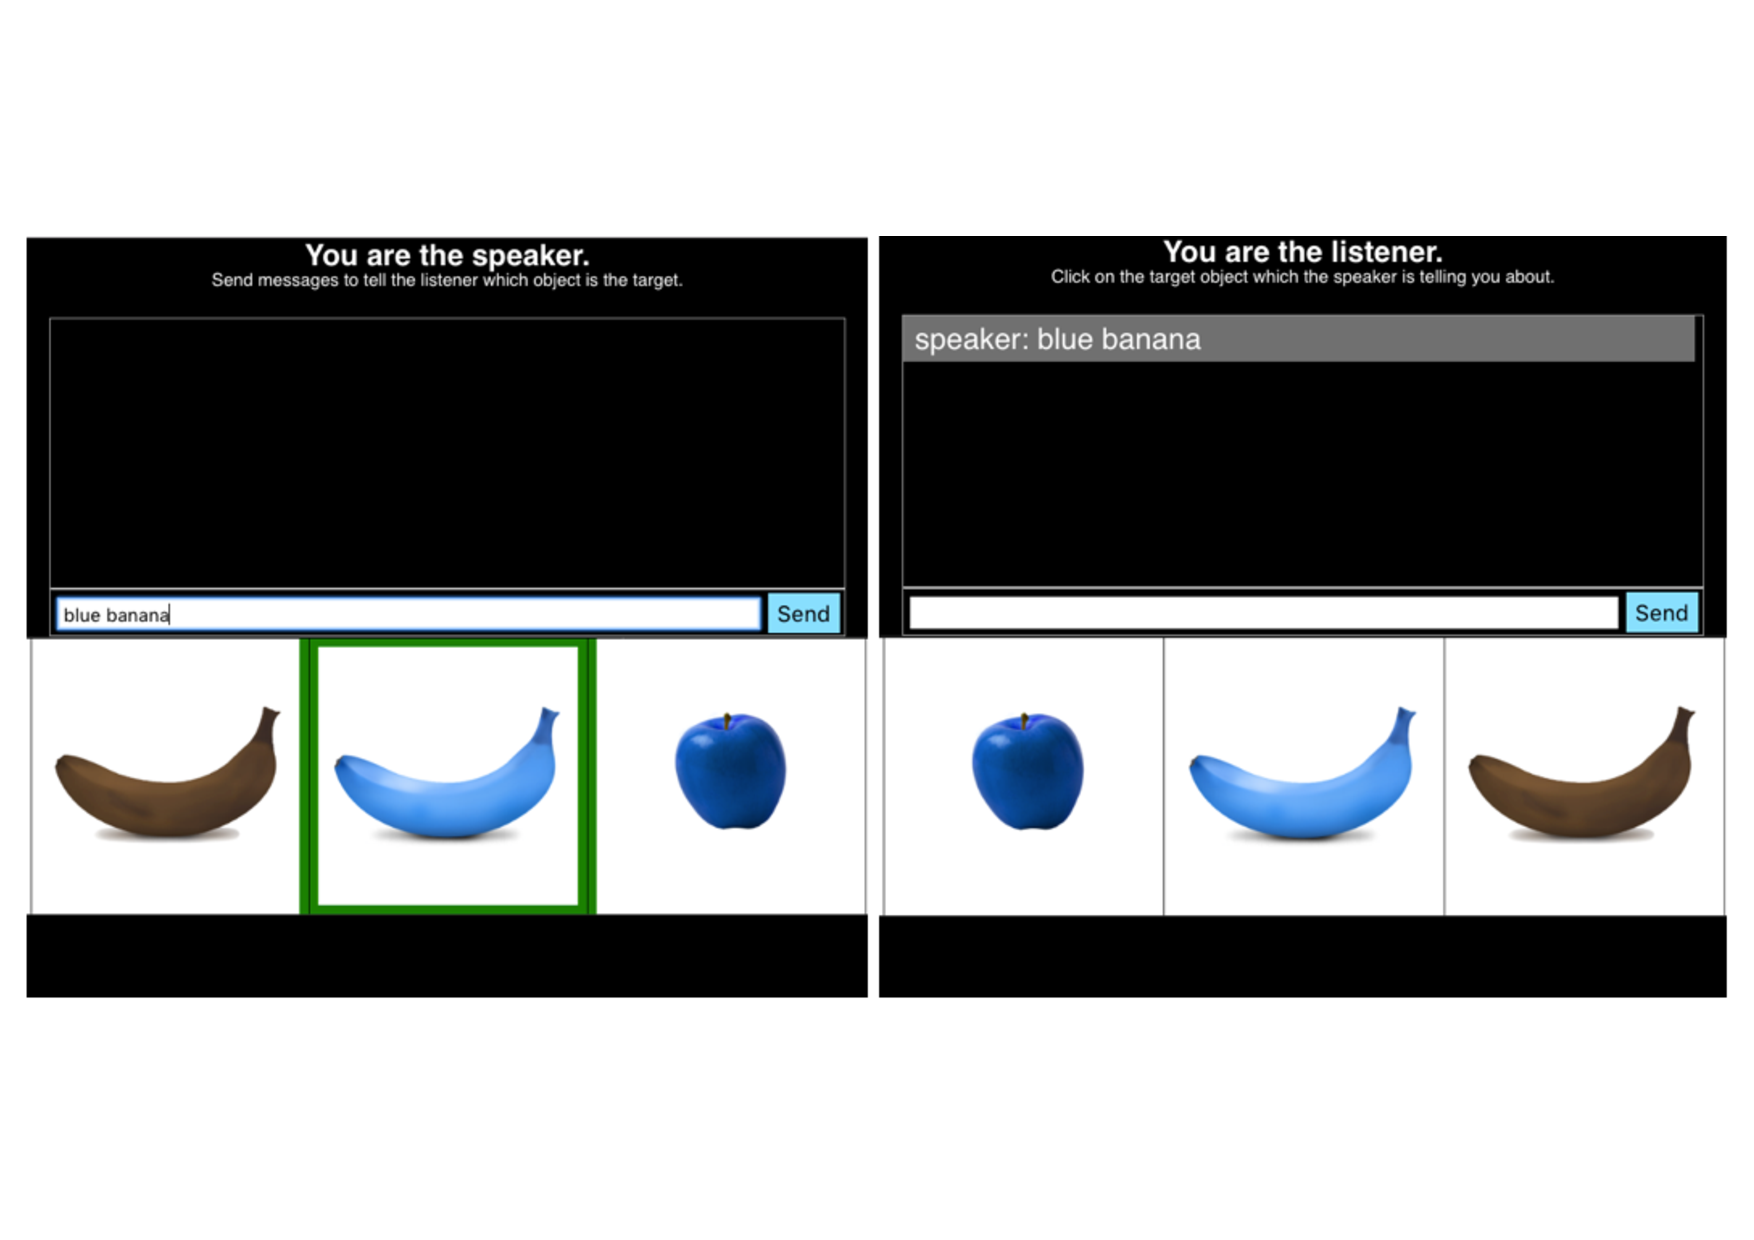
\includegraphics[width=.5\textwidth]{graphs/design_0}
	\caption{Experimental setup.
	}
	\label{fig:mturk}
\end{figure}

%\subsection{Methods}

\subsection{Participants and materials}
We recruited 120 self-reported native speakers of English over Mechanical Turk. The experiment was a multi-player reference game in which one participant was randomly assigned to the role of the speaker, and the other one to the role of the listener. The speaker's task was to communicate a target object out of three-object contexts to the listener. The target was always marked with a green border (see \figref{fig:mturk}). The listener clicked on the object they thought was the target. The speaker and the listener could communicate freely through a chat box.

%\paragraph{\bf Materials}
The stimuli were selected from seven food items (apple, avocado, banana, carrot, pear, pepper, tomato) which each occurred in three different colors that intuitively differed in typicality for that item. For example, the banana occurred in the colors yellow, brown, and blue. Each item occurred as a target and as a distractor. A pepper additionally occurred in a fourth color which only functioned as a distractor due to the need for a green color competitor.

%\paragraph{\bf Design}
Each presented context consisted of three objects, one target and two distractors. The contexts always corresponded to one out of four possible conditions. The different context conditions are referred to as ``informative without a color competitor" (Fig.~1a), ``informative with a color competitor" (Fig.~1b), ``overinformative without a color competitor" (Fig.~1c), and ``overinformative with a color competitor" (Fig.~1d). A context is referred to as overinformative when mentioning the type of the item, e.g., banana, would be sufficient for an unambiguous identification of the target. An additional mention of color would mean that the speaker uses the color adjective overinformatively, i.e., they are adding ``unnecessary" information. However, in this condition the target never has a color competitor, i.e., if the target is brown, there is no distractor of the same color in the context. This means that an only-color utterance would lead to an unambiguous identification, too. This is not possible in the overinformative condition with a color competitor (Fig.~1d). In the informative conditions, the speaker needed to mention the color in addition to the type to provide an unambiguous utterance. Again, one context type did (Fig.~1a) and one did not include a color competitor among its distractors (Fig.~1b).

The item selection was randomized but conditioned on the corresponding context condition, i.e., the items had to fulfill the properties dictated by the condition. In the end, each participant saw 42 different contexts. All of the differently colored items were the target exactly twice but the context in which they occurred was drawn randomly from the four possible conditions mentioned above. All in all, there were 84 different configurations, i.e., seven target food items, each of them in three colors, where each could occur in four contexts. Trial order was randomized.


\subsection{Procedure}

Participants were randomly paired up and each was randomly assigned either to the role of  speaker or listener. They communicated through a real-time multi-player interface as described in \citeA{Hawkins15_RealTimeWebExperiments}. The virtual environment of the experiment can be seen in \figref{fig:mturk}. The speaker and the listener saw the same set of objects but in a randomized order to avoid trivial position-based references such as ``the left one". After the listener clicked on the presumed target, both speaker and listener received feedback about whether the right object had been selected.


\subsection{Annotation}
After collecting the data, the different utterances were labeled as belonging to one of the following categories: type-only ("banana"), color-and-type ("yellow banana"),  color-only ("yellow"), category-only ("fruit"), color-and-category ("yellow fruit"), description ("has green stem"), color-modifier ("funky carrot"), and negation ("yellow but not banana"). Before sorting, two participants were excluded because they did not finish the experiment. Trials on which the speaker did not produce any utterances and trials on which the listener did not identify the target correctly were excluded as well. The remaining utterances (94\% of the original set) were cleaned manually for misspellings and abbreviations, e.g., ``banan" for banana. Finally, there were XX \jd{elisa: how many??} speakers  who consistently used roundabout descriptions instead of direct referring expressions (e.g., "monkeys love..." for banana). These participants were excluded because they were clearly not trying to simply communicate the target.

The 1942 resulting utterances were then categorized according to the categories laid out above. Only five utterances (0.003\%) were assigned to the category "other".

%\begin{figure}[bt!]
%	\centering
%	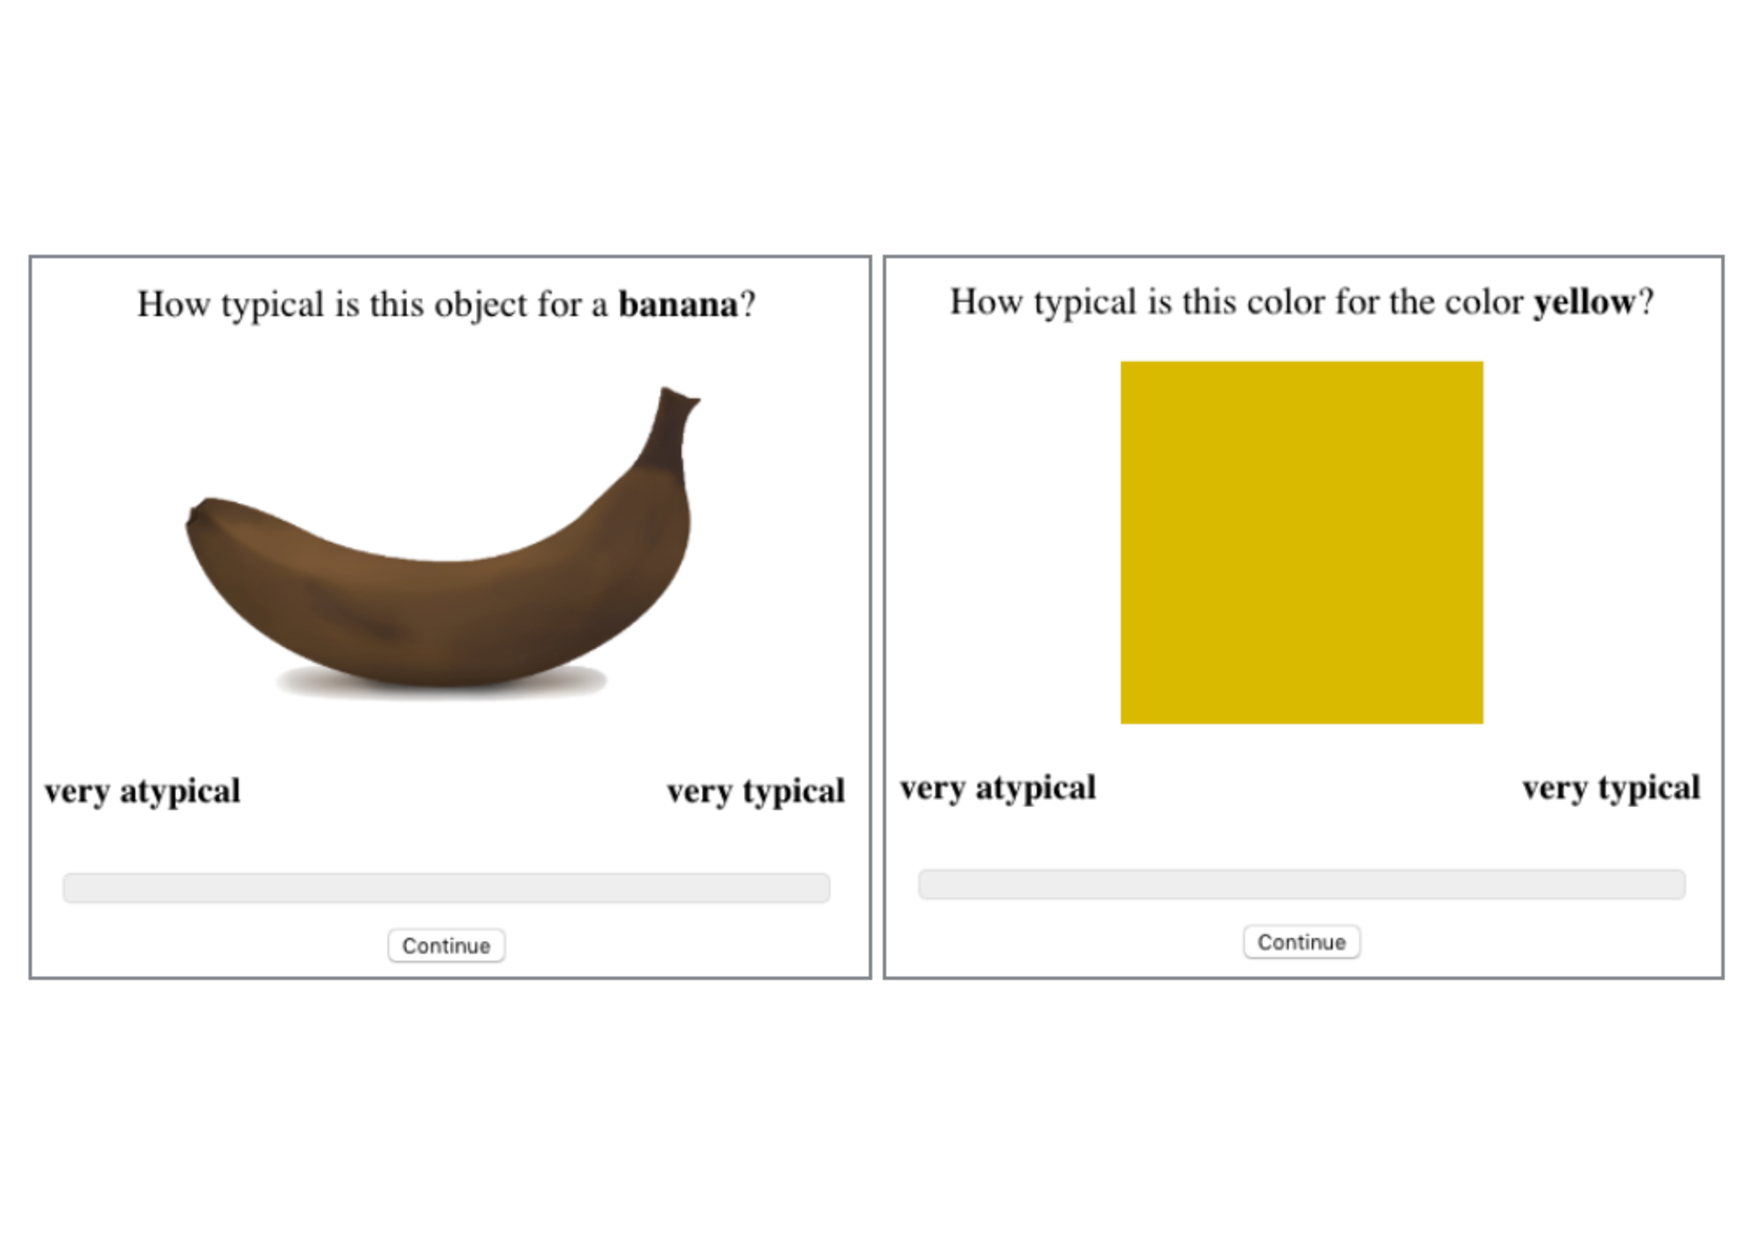
\includegraphics[width=.5\textwidth]{graphs/design_2}
%	\caption{Typicality norming studies for object and color patch norming.
%	}
%	\label{fig:design_2}
%\end{figure}



\subsection{Typicality norming}

To evaluate the model we report below, we collected empirical typicality values for each utterance-object pair. Ratings were collected across three separate studies. The first study collected typicalities for adjective\&noun-object pairs, e.g., ``yellow banana'' as applied to a yellow banana, a blue banana, an orange pear, etc. The second study collected typicalities for noun-object pairs, e.g., ``banana'' as applied to a yellow banana, a blue banana, an orange pear, etc. The third study collected typicalities for adjective-color pairs, e.g., ``yellow'' as applied to a color patch of the average yellow from the yellow banana image or to a color patch of the average orange from the orange pear image.  On each trial, participants saw one of the images used in the production experiment in isolation and were asked: ``How typical is this object for a \textsc{utterance}'', where \textsc{utterance} was replaced by an utterance of interest. In the color typicality study, they were asked ``How typical is this color for the color \textsc{color}?'', where \textsc{color} was replaced by one of the relevant color terms.  They then adjusted a sliding scale with endpoints labeled ``very atypical'' and ``very typical'' to indicated their response. A screenshot of a typical trial is shown in \figref{fig:typicalitynorming}. An overview of the differences between the three typicality norming studies differed is shown in \tableref{tab:normingoverview}. Each participant saw each `correct' combination of utterances and objects (22 total) as well as a number of randomly sampled trials from the total set of items in each study, shown in the table.

\begin{figure}[bt!]
	\centering
	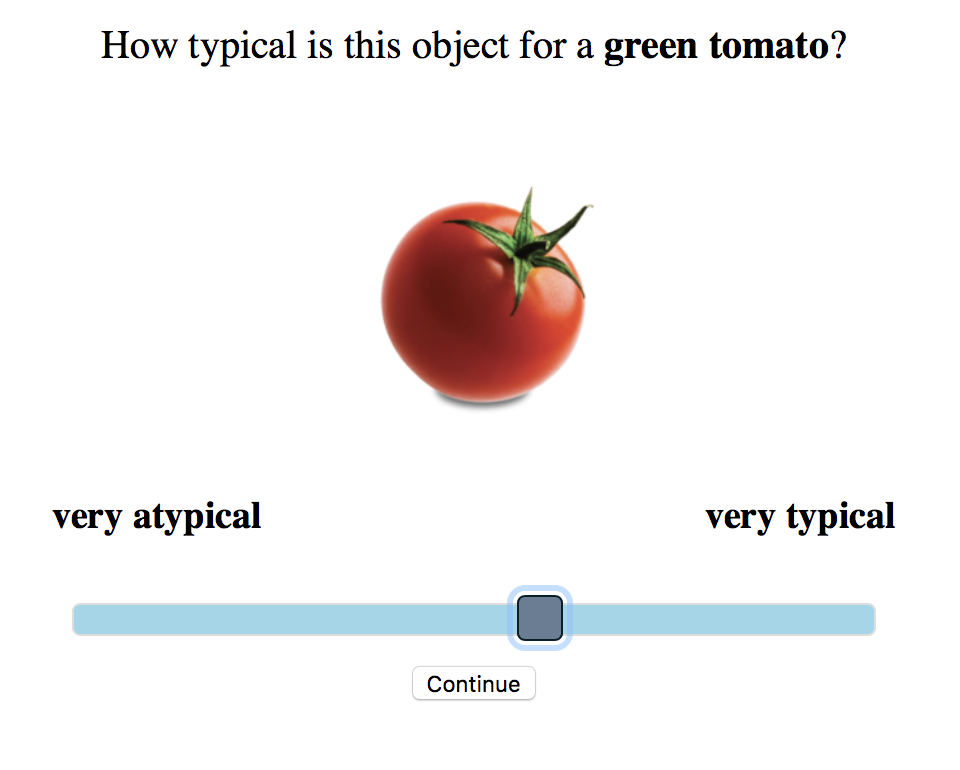
\includegraphics[width=.5\textwidth]{graphs/typ_norm_full_2}
	\caption{A typical trial in the `Adj Noun' typicality norming study.
	}
	\label{fig:typicalitynorming}
\end{figure}


\begin{table*}
\caption{Overview of typicality norming studies.}
\begin{tabular}{l l l l l l l}
\toprule
Utterances & Example & Images & Participants & Trials & Items & Excluded\\
\midrule
Adj Noun & \emph{yellow banana} & object & \jd{elisa, fill in} & 110 & 484 & \jd{elisa, fill in}\\ 
Noun & \emph{banana} & object & \jd{elisa, fill in} & 90 & \jd{elisa, fill in} & \jd{elisa, fill in}\\
Adj & \emph{yellow} & color patch & \jd{elisa, fill in} & 90 & \jd{elisa, fill in} & \jd{elisa, fill in}\\
\bottomrule
\end{tabular}
\label{tab:normingoverview}
\end{table*}

Slider values were coded as falling between 0 (`very atypical') and 1 (`very typical'). For each utterance-object combination we computed mean typicality ratings. For example, mean typicalities for the banana items are shown in \tableref{tab:bananatypicalities}.

\begin{table}
\caption{Mean typicalities for banana items. Combinations where a deterministic semantics would return TRUE are marked in boldface.}
\begin{tabular}{r r r r r}
\toprule
%Utterance & Item & Typicality\\
 & \multicolumn{3}{c}{Banana items} & Other \\
 Utterance & yellow & brown  & blue & \\ 
 \midrule
\emph{banana} & \textbf{.98} & \textbf{.66} & \textbf{.42} & .05  \\
 \midrule
\emph{yellow banana} & \textbf{.98} & .33 & .17 & .05 \\
\emph{brown banana} & .28 & \textbf{.90} & .18 & .04\\
\emph{blue banana} & .20 & .18 & \textbf{.91} & .06\\
\bottomrule
\end{tabular}
\label{tab:bananatypicalities}
\end{table}

%66 participants  were recruited via Mechanical Turk. Two participants were excluded because they were not self-reported English speakers, and two because their responses were random. \jd{measured how?}
%
%They were shown a colored food item, e.g., a blue banana, and asked "How typical is this object for an X?" (X being a color-type combination, e.g., blue banana, or red apple). The participants could rate the fitness on a continuous draggable scale from "very atypical" to "very typical". Every object in the set was paired with every color-type combination from the set, resulting in 484 different trials. Each participant answered 110 trials in which type consistent trials (showing all kinds of bananas when utterance contains the word banana) were always present, and non-fitting trials which were selected randomly. The amount of data per combination ranged from 1 to 62. The assumed typicality values are the averaged slider values for each combination ranging from 0 (very atypical) to 0.983 (very typical). 

The way we elicited typicalities differs somewhat from the approach taken in previous work \cite<e.g.>{westerbeek2015}, where participants are typically asked ``How typical is this color for this object?'' We deviated from this because for the purpose of testing the model (see below), what is required is the degree of applicability of an utterance to an object, rather than the degree to which an object's color is representative of that object. We expect, however, that the simple noun-object typicalities will yield very similar results as the Westerbeek question because the employed objects are color-diagnostic -- asking whether an blue or a yellow banana is a typical \emph{banana} is similar to asking whether or not the bananas' most salient property -- their color -- is typical. 

\subsection{Results and discussion}

Proportions of type-only (\emph{banana}), color-and-type (\emph{yellow banana}), color-only (\emph{yellow}), and other (\emph{funky carrot}) are shown in \figref{fig:proportions}. Visually inspecting just the explicitly marked \emph{yellow banana}, \emph{brown banana}, and \emph{blue banana} cases suggests a clear typicality effect in the overinformative conditions as well as a smaller typicality effect in the informative conditions. 

\begin{figure}[bt]
\centering
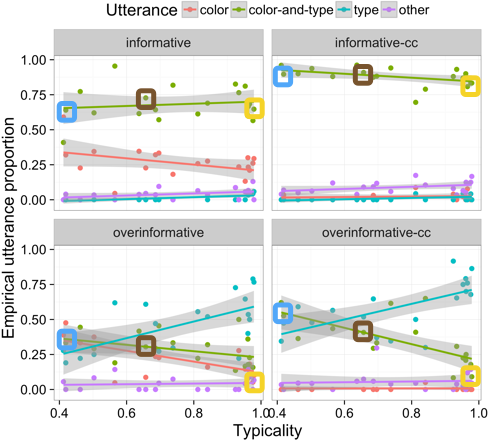
\includegraphics[width=.5\textwidth]{graphs/results1.png}
\caption{For each target, proportion of color-only (\emph{yellow}), type-only (\emph{banana}), color-and-type (\emph{yellow banana}), and other (\emph{funky carrot}) utterances as a function of mean object typicality for the type-only utterance, across conditions. \emph{\textsc{color} banana} cases are circled in their respective color.}
\label{fig:proportions}
\end{figure}

The following questions are of interest. First, do we replicate the previously documented typicality effect on redundant color mention beyond the one-item visual inspection? Second, do we observe typicality effects even when color is informative (i.e., technically necessary for establishing unique reference)? Third, are speakers sensitive to the presence of color competitors in their use of color or are typicality effects immune to the nature of the distractor items?

To address these questions we conducted a mixed effects logistic regression predicting color use from fixed effects of typicality, informativeness, and color competitor presence. We used the typicality norms obtained in the noun-object typicality elicitation study reported above as the continuous typicality predictor. Informativeness was coded as a binary variable (color \emph{informative} vs.~color overinformative) as was color competitor presence (absent vs.~present). All predictors were centered before entering the analysis. The model included by-speaker and by-item random intercepts, which was the maximal random effects structure that allowed the model to converge.

There was a main effect of typicality, such that the more typical an object was for the noun, the lower the log odds of color mention ($\beta$ = -3.19, $SE$ = 0.36, $p <$ .0001), replicating previously documented typicality effects. Model comparison revealed that including interaction terms was not justified by the data, suggesting that speakers produce more typical colors less often even when the color is in principle necessary for establishing reference (i.e., in the informative conditions). There was also a main effect of informativeness, such that color mention was more likely when it was informative than when it was overinformative   ($\beta$ = 3.32, $SE$ = 0.16, $p <$ .0001). Finally, there was a main effect of color competitor presence, such that color mention was less likely when a color competitor was present  ($\beta$ = -0.66, $SE$ = 0.13, $p <$ .0001). This suggests that speakers are indeed sensitive to the contextual utility of color -- color typicality alone does not capture the full set of facts about color mention.

In this section we have reported the replication of previously documented typicality effects on color mention as well as a novel demonstration of typicality effects even when color is informative. We have also shown that color mention is sensitive not only to typicality, but also to the  nature of the distractors -- when there is another distractor of the same color as the target, color is dispreferred compared to when there is not. 
%What this suggests is that choosing to include a color modifier in a referring expression is not just a function of one factor. While it is clear that 
Thus far we have only been concerned with analyzing the use of color, i.e., we collapsed \textsc{color} and \textsc{color-and-type} utterances into one category. However, our goal is to formulate a cognitive model that captures the production of referring expressions more generally. To this we turn next.

\section{Modeling referential expressions}

We consider a family of computational models characterizing the communicative challenge a speaker agent faces in the reference game scenarios above. These models are all situated within the broader Rational Speech Act (RSA) framework, which has successfully explained a range of sophisticated language phenomena through a recursive process of social reasoning between speaker and listener agents \cite{frank2012, goodmanstuhlmueller2013, GoodmanFrank2016}. More formally, we define a \emph{literal listener} $L_0$ that selects between contextual referents $c \in \mathcal{C}$ proportionally to the meanings given by a lexicon $\mathcal{L}$:

$$L_0(c | u, \mathcal{C}) \propto \mathcal{L}(u, c) P(c)$$

We assume uniform prior beliefs $P(c)$ over referents. We then introduce a pragmatic speaker $S_1$, which selects an utterance $u \in \mathcal{U}$ to communicate an intended referent $c_i$ by trading off \emph{informativity} with \emph{cost}:
%%%
$$S_1(u | c_i) \propto \exp\left( \alpha\log(L_0(c_i | u, \mathcal{C})) - \textrm{cost}(u) \right)$$
%%%
where cost is usually defined as a function of an utterance's length or corpus frequency \jd{make sure we report the right cost function in final version} and $\alpha$ is a parameter controlling the speaker's ``optimality'': as $\alpha\rightarrow \infty$, they will choose utterances that maximize informativity. We explore several variations of this model in our model comparison, first considering different formulations of the lexicon $\mathcal{L}$ and then  several novel ways of enriching the speaker to marginalize over possible \emph{noise} in the listener's perception of the context:

\subsection{Model alternatives}

\paragraph{Baseline:} The simplest version of the lexicon $\mathcal{L}$ uses truth-conditional meanings, such that a given utterance is either true or false of a given referent: $\mathcal{L}(u,c) = \delta_{u(c)}$. This is the traditional formulation in formal semantics, and the one most frequently used in previous RSA models. 

\paragraph{Typicality:} \jd{Motivate with banana example?} Next, we consider the elaborated model in \citeA{GrafEtAl2016}, which focused on nominal reference contexts where a speaker must choose between different taxonomic levels of reference (e.g. `dalmatian,' `dog,' or `animal'). The primary innovation introduced by \citeA{GrafEtAl2016} was a shift to a graded, real-valued meaning function based on the \emph{typicality} of the referent relative to the utterance category: $\mathcal{L}(u,c) = \textrm{typicality(u, c)}$. This gives rise to phenomena where, for example, a speaker is more likely to use an overinformative utterance for a particularly atypical category member when a more typical referent is in context because they reason that $L_0$ would interpret the simpler utterance to mean the more typical referent. In the color typicality contexts we examine here, this corresponds to speakers being more likely to use an overinformative color-and-type utterance for  a particularly  atypical category member (blue banana) when there are other objects present that receive greater-than-zero  typicality for the unmodified noun (\emph{banana}) compared to when the target item is instead a highly typical category member (yellow banana). 

\paragraph{Uniform Perceptual Noise:} An additional source of uncertainty in language production comes from considerations of perceptual noise \cite<in the speaker or in the listener,>{jaeger2010}. We propose that perceptual noise is another critical factor in explaining the overproduction of redundant modifiers. In this variation of the model, the speaker supposes that with some noise parameter $p_{noise}$, the listener might have misperceived one or more of the objects in context, thus leading to a corrupted context $\mathcal{C}'$:
$$S_{noisy}(u|c_i) \propto \exp\left( \alpha\log\left(\sum_{\mathcal{C'}} P(\mathcal{C}')L_0(c_i | u, \mathcal{C}')\right) - \textrm{cost}(u)\right)$$
In the simplest version of this noisy-context model, the prior over possible misperceptions $P(\mathcal{C}')$ is uniform, such that the true context has probability $P(\mathcal{C}) = p_{noise}$, and the rest of the probability mass is spread evenly across all possible replacements of one or more objects $c \in \mathcal{C}$. Intuitively, this has the effect of making the speaker more cautious about using less specific utterances: even if there is only one `banana' in context, the speaker reasons that the listener may misperceive one of the distractors as another banana with some small probability, hence it may be useful to include a color modifier just in case.

\paragraph{Similarity-Based Perceptual Noise:} This model is equivalent to the Uniform Perceptual Noise except for the prior $P(\mathcal{C'})$ over possible corruptions. Rather than choosing uniform across possible corruptions, we define a similarity metric such that misperceptions closer in similarity space to the true context (e.g. sharing one or more complete objects, only differing in color, and so on) are proportionally more likely: $P(\mathcal{C'}) \propto \textrm{sim}(\mathcal{C}, \mathcal{C'})$.
\rdh{Need to explain this similarity metric more once we've settled on one}
%\end{description}

%The ghost-context model is similar to the simple model, but adds uncertainty by taking the true context and creating possible variants from it in a random fashion. This contributes the possibility of a misperception. Possible contexts that are more similar to the true context appear with a higher probability than those with a lower one. Here, similarity is only calculated on basis of the whole object (color and type) being identical to its corresponding partner in the true context
%This model also has an extended version in which the similarity measure is more fine-grained, i.e., color is not a binary feature anymore (either true or false) but rather can be more or less similar to the color of the object in the true context.



\subsection{Model evaluation}

\jd{waiting for results\dots -- what we'll want is a faceted scatterplot of all the model posterior predictives we end up comparing plus ca. 2 paragraphs of discussion}


%
%We formulated a probabilistic model of reference level selection that integrates contextual informativeness, utterance cost, and typicality.
%As in earlier Rational Speech-Acts (RSA) models \cite{frank2012, goodmanstuhlmueller2013}, the speaker seeks to be informative with respect to an internal model of a literal listener. This listener updates her beliefs to rule out possible worlds that are inconsistent with the meaning of the speaker's utterance. Rather than assuming that words have deterministic truth conditions, as has usually been done in the past, we account for typicality by allowing each label a graded meaning. For instance, the word ``dog'' describes a dalmatian better than a grizzly bear, but it also describes a grizzly bear better than a tennis ball.
%The speaker also seeks to be parsimonious: the speaker utility includes both informativeness and word cost; cost includes both length and frequency.
%
%Formally, we start by specifying a literal listener $L_0$ who hears a word $l$ at a particular level of reference  in the context of some set of objects $\mathcal{O}$ and forms a distribution over the referenced object, $o \in \mathcal{O}$ : 
%$$P_{L_0}(o | l) \propto \denote{l}(o).$$
%Here $\denote{l}(o)$ is the lexical meaning of the word $l$ when applied to object $o$. We take this to be a real number indicating the degree of acceptability of object $o$ for category $l$. 
%We relate this to our empirically elicited typicality norms via an exponential relationship: $\denote{l}(o)=\exp(\text{typicality}(o,l))$.\footnote{Cases where typicality was not elicited were assumed to have typicality $0$.}
%This relationship is motivated by considering the effect of a small difference in typicality on choice probability: in our elicitation experiment a small difference in rating should mean the same thing at the top and bottom of the scale (it is visually equivalent on the slider that participants used).
%In order for a small difference in typicality rating to have a constant effect on relative choice probability (which is a ratio), the relationship must be exponential. 
%Next, we specify a speaker $S_1$ who intends to refer to a particular object $o \in \mathcal{O}$ and chooses among possible nouns $l \in {\mathcal L}(o)$.
%We take ${\mathcal L}(o)$ to be the three labels for $o$ at sub, basic, and super level.
%The speaker chooses among these nouns in a way that is influenced by informativeness of the noun for the literal listener ($\ln P_{L_0}(o | l)$), the frequency ($\hat{c}_f$) and the length  ($\hat{c}_l$), each weighted by a free parameter:
%$$P_{S_1}(l | o) \propto \exp(\lambda \ln P_{L_0}(o | l) + \beta_f \hat{c}_f  + \beta_l \hat{c}_l)$$
%Length cost $\hat{c}_l$ was defined as the empirical mean number of characters used to refer at that level and frequency cost $\hat{c}_f$ was the log frequency in the Google Books corpus from 1960 to the present. 
%
%We performed Bayesian data analysis to generate model predictions, conditioning on the observed production data (coded into sub, basic, and super labels as described above) and integrating over the three free parameters.
%We assumed uniform priors for each parameter: $\lambda  \sim Unif(0,20)$, $\beta_f \sim Unif(0,5)$, $\beta_l \sim Unif(0,5)$.
%We implemented both the cognitive and data-analysis models in the probabilistic programming language WebPPL \cite{GoodmanStuhlmuller14_DIPPL}.
%Inference for the cognitive model was exact, while we used Markov Chain Monte Carlo (MCMC) to infer posteriors for the three free parameters.

%\begin{figure}[t!]
%\centering
%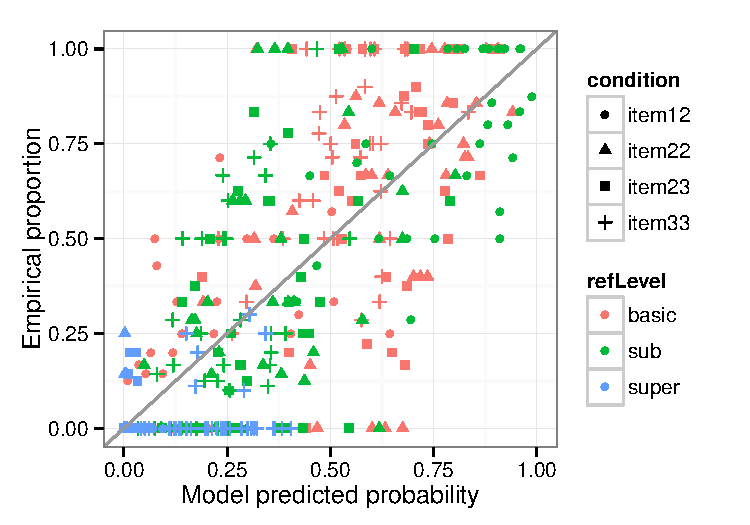
\includegraphics[width=.5\textwidth]{graphs/scatterplot}
%\caption{Mean empirical production data for each level of reference against the MAP of the model posterior predictive at the by-target level.}
% \label{fig:scatterplot}
%\end{figure}

%Point-wise maximum a posteriori (MAP) estimates of the model's posterior predictives at the target level (collapsing across distractors for each target, within each condition) are compared to empirical data in Fig.~\ref{fig:scatterplot}. On the by-target level the model achieves a correlation of $r = .79$. Looking at results on the by-domain level (collapsing across targets) and on the by-condition level (further collapsing across domains, as in \figref{fig:qualitativemodel}) yields correlations of .88 and .96, respectively. 
%The model does a good job of capturing the quantitative patterns in the data, especially considering the sparsity of our data at the by-target level.
%One clear flaw is that the model predicts greater use of the super level label than people exhibit.
%Further systematic deviation appears likely for specific items. 
%On examination, candy items like ``gummy bears'' or ``jelly beans'' were particularly problematic, being referred to primarily by their sub level term in all contexts.

%\begin{figure}
%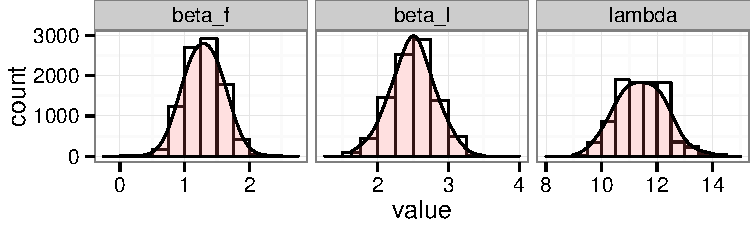
\includegraphics[width=.49\textwidth]{graphs/parameterposteriors.pdf}
%\caption{Posterior distribution over model parameters. Maximum a posteriori (MAP) $\lambda = 10.8$, 95\% highest density interval (HDI) $= [9.7, 12.8]$; MAP $\beta_l = 2.5$, HDI $= [1.9, 3.1]$; MAP $\beta_f = 1.3$, HDI $= [0.8, 1.8]$.}
%\label{fig:paramposteriors}
%\end{figure}

%Parameter posteriors are presented in Fig.~\ref{fig:paramposteriors}. 
%Informativeness is weighted relatively strongly, while length is weighted somewhat more strongly than frequency.
%Note that the 95\% highest density intervals (HDIs) for all three weight parameters exclude zero, indicating that some contribution of each is useful in explaining the data.
%In order to ascertain whether typicality was indeed contributing to the explanatory power of the model, we ran an additional Bayesian data analysis with an added typicality weight parameter $\beta_t \in [0,1]$. This parameter interpolated between empirical typicality values (when $\beta_t {=} 1$) and deterministic (i.e. $0$ or $1$) \emph{a priori} values based on the true taxonomy (when $\beta_t {=} 0$).
%We found a MAP estimate for $\beta_t$ of $.94$, HDI $= [0.88,1]$, strongly indicating that it is useful to incorporate empirical typicality values.
%Finally, we ran a model including a parameter weighting the \emph{product} of frequency and cost, corresponding to the interaction term in our regression analysis. Its posterior distribution was strongly peaked at 0, indicating that any contribution of the interaction is already captured by other aspects of the model. 



\section{Discussion and conclusion}

The work reported here makes both empirical and theoretical contributions. Empirically, we both replicated previously reported color typicality effects on the production of `overinformative' referring expressions \cite{sedivy2003a, westerbeek2015, rubiofernandez2016} and demonstrated unexpected color typicality effects on the production of `informative' referring expressions as well: even when color is necessary for reference because a distractor object of the same category is present, color is sometimes dropped if the distractor is particularly atypical -- i.e., speakers will sometimes refer to a yellow banana in the context of a blue banana simply as a \emph{banana}. Theoretically, we have provided a unified account of color typicality effects in language production within the Rational Speech Act framework \cite{GoodmanFrank2016} with graded rather than deterministic semantics. The best-fitting model \jd{add a sentence on its characteristics and why it was the most successful, using a qualitative example}.

While the modeling reported here constitutes an intriguing extension of a graded-semantics RSA model from the nominal \cite{GrafEtAl2016} to the modified NP domain, there remain a number of interesting open questions for future research. First and foremost, while we have shown that computing an utterance's contextual informativeness using empirically elicited typicalities for one-word and two-word utterances yields precisely the kinds of noisy literal listener distributions that pragmatic speakers seem to consider, it is an open question how the two-word typicalities are come by compositionally. That is, given the typicalities of the one-word utterances (e.g., \emph{banana} and \emph{blue}), what is the right way of combining these to arrive at the appropriate two-word utterance typicalities for a particular object? This is a question that has received attention time and time again whenever a non-deterministic semantics is considered \cite{Kamp1995}. Given the tools at hand, we are now in a position to formally test multiple hypotheses about the compositional semantics of terms with continuous meanings. This is an exciting avenue for future research.

\jd{discuss perceptual noise models vs typicality semantics models? ie different kinds of uncertainty}

\jd{add concluding sentence}

%to get a more intuitive model: tried to compute typicalities for an object given a particular utterance by taking the value of how good that particular color is as an instance of that color, and the typicality of that object as an instance of the object's type. In other words, if there is a blue banana how blue is this particular blue and how good of an instance is this blue banana for a banana.




\section{\bf Acknowledgments}
\small
This work was supported by ONR grant N00014-13-1-0788 and a James S. McDonnell Foundation Scholar Award to NDG. RXDH was supported by the Stanford Graduate Fellowship and the National Science Foundation Graduate Research Fellowship under Grant No. DGE-114747.



\bibliographystyle{apacite}

\setlength{\bibleftmargin}{.125in}
\setlength{\bibindent}{-\bibleftmargin}

\bibliography{bibs}


\end{document}